\section{Ontology-based Streaming Data Access}
\label{approach}


%\begin{itemize}
%\item establishing mappings between global ontological models and streaming data source schemas.
%\item accessing streaming data sources through queries over ontology global models.
%\item integrating streaming and stored data sources through an ontological unified view.
%\item combining data from event-based streams and/or sensor networks acquisitional streams considering time and tuple windows.
%\item considering quality-of-service requirements for query optimisation and source selection during the integration.
%\end{itemize}

\begin{figure}[t]
  \centering
  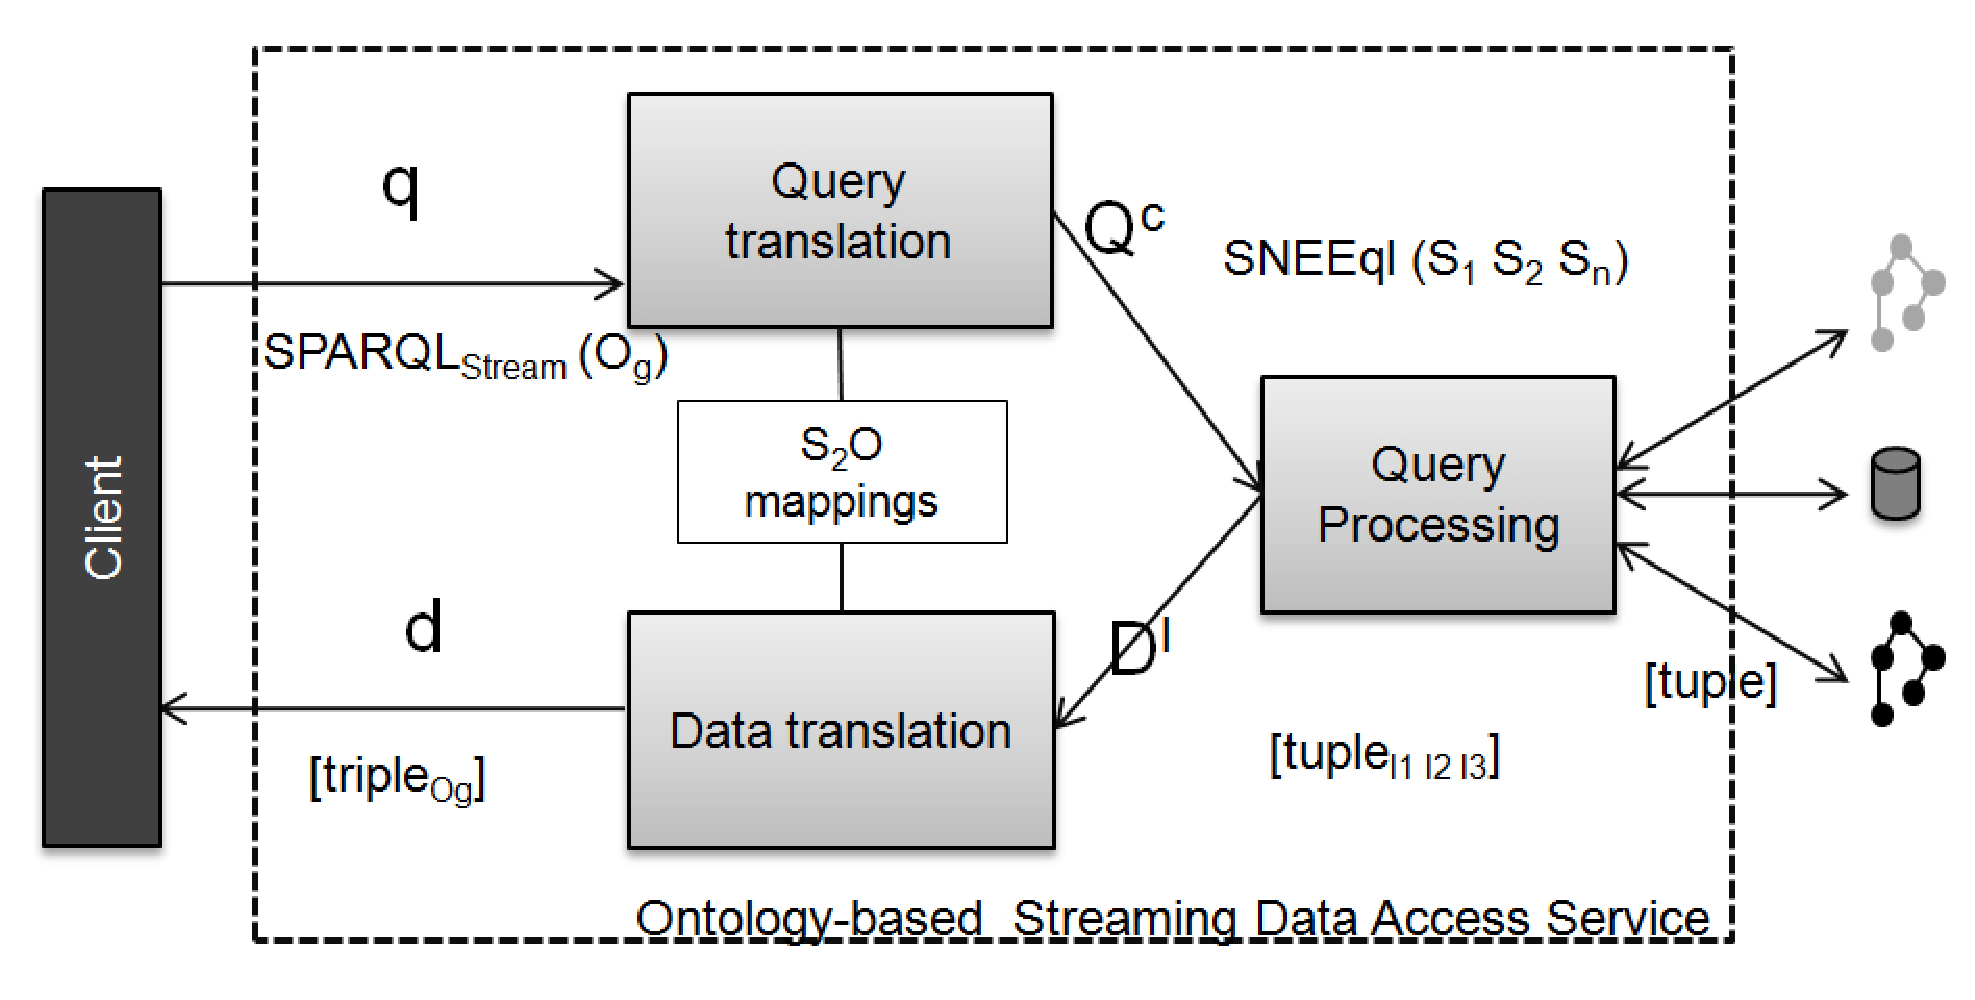
\includegraphics[width=.8\textwidth]{img/approachImg}
  \caption{Ontology-based streaming data access service} 
  \label{fig:SemanticIntegrator} 
\end{figure}

Our approach to enable ontology-based access to streaming data is depicted in Fig~\ref{fig:SemanticIntegrator}.\ %  that can receive requests over an ontological view and transforms them into queries for acquisitional or event-based stream sources or stored sources. The results of these queries can be integrated following a query plan and returned as RDF triples in terms of the global ontology. The approach is depicted in Fig ~\ref{fig:SemanticIntegrator}.
The service receives queries specified in terms of the classes and properties\footnote{We use the \owl nomenclature of classes, and object and datatype properties for naming ontology elements.} of the ontology using \sparqlstr, an extension of \sparql that supports operators over \rdf streams (see Section~\ref{streamingsparqlsyntax}). 
In order to transform the \sparqlstr query, expressed in terms of the ontology, into queries in terms of the data sources, a set of mappings must be specified. 
These mappings are expressed in \stwoo, an extension of the \rtwoo mapping language, which supports streaming queries and data, most notably window and stream operators (see Section~\ref{streamingr2osyntax}). 
This transformation process is called \textit{query translation}, and the target is the continuous query language \sneeql, which is expressive enough to deal with both streaming and stored sources.

After the continuous query has been generated, the query processing phase starts, and the processor will deploy distributed query processing techniques~\cite{Kossmann_00} to extract the relevant data from the sources and perform the required query processing, \eg selection, projection, and joins. %creating a query plan that indicates how the sources will be accessed and how the data will be joined and combined using the available operators\cite{Kossmann_00}.no
%
Note that query execution in sources such as sensor networks may include in-network query processing, delivery of data between sources may be pull or push based, and other data source specific settings. The result of the query processing is a set of tuples that the \textit{data translation} process transforms into ontology instances.

This approach requires several contributions and extensions to the existing technologies for continuous data querying, ontology-based data access, and \sparql query processing. 
This paper focuses on a first stage that includes the process of transforming the \sparqlstr queries into queries over the streaming data sources using \sneeql as the target language.
The following sections provide the syntax and semantics for the querying of streaming \rdf data and the mappings between streaming sources and an ontology.
We will then provide details of an implementation of this approach.

%%% Local Variables: 
%%% mode: latex
%%% TeX-master: "rere"
%%% End: 
